\chapter{哈密顿-雅可比理论}
\label{ch:6}

\section*{6.1 哈密顿-雅可比方程}

一个动力学问题，当我们在给定初始条件和时间的情况下确定了广义坐标与广义动量之间的关系时，便算得到了解决。初始条件可以表示为 $q_0$ 和 $p_0$，这里我们指的是坐标 $q_i$ 和动量 $p_i$ 在 $t = 0$ 时刻的常数值。力学问题的解是一组关系式
\[
q = q(q_0, p_0, t), \tag{6.1}
\]
\[
p = p(q_0, p_0, t).
\]
这些方程可以看作是在正则变量 $q$、$p$ 与一组新变量 $q_0$、$p_0$ 之间的变换方程。求解力学问题等价于找出从 $q$、$p$ 到 $q_0$、$p_0$ 的变换。但 $q_0$、$p_0$ 是常数；因此我们需要找出一个从正则变量 $(q, p)$ 到一组常数的变换。我们现在来表明如何做到这一点。

正则变换把我们由哈密顿量 $H = H(p, q, t)$ 变换到变换后的哈密顿量 $K = K(P, Q, t)$，其中
\[
\dot{Q}_i = \frac{\partial K}{\partial P_i},
\]
\[
\dot{P}_i = -\frac{\partial K}{\partial Q_i},
\]
以及
\[
K = H + \frac{\partial F}{\partial t}.
\]
如果新变量是常数，我们就有 $\dot{Q}_i = 0$ 和 $\dot{P}_i = 0$。（我们希望这些"新"变量是坐标和动量的恒定初始值。）要求新变量为常数，只需简单地要求 $K$ 为常数即可保证。事实上，如果我们令 $K = 0$，那么显然 $\dot{Q}_i = 0$ 且 $\dot{P}_i = 0$。令 $K = 0$ 得到
\[
H + \frac{\partial F}{\partial t} = 0. \tag{6.2}
\]
这是一个可以解出 $F$ 的微分方程。（回忆 $F$ 是正则变换的生成函数。）

我们将选取 $F$ 具有 $F = F_2(q, P, t)$ 的形式。这是一个合理的选择，因为这个生成函数把我们由 $p$ 变换到 $P$，由 $q$ 变换到 $Q$。你还会记得，这正是无穷小接触变换的基础，这些接触变换把一个时刻的 $q$ 和 $p$ 带到另一时刻的 $q$ 和 $p$。

我们先前用 $F_2$ 表示这个生成函数，但现在，出于历史原因，我们改用 $S$ 表示。我们（尚）不知道 $S$ 的函数形式，但我们知道
\[
S = S(q, P, t).
\]
在哈密顿-雅可比理论中，函数 $S$ 被称为哈密顿主函数。

由方程（5.14）
\[
p_i = \frac{\partial S}{\partial q_i}, \tag{6.3}
\]
\[
Q_i = \frac{\partial S}{\partial P_i},
\]
\[
K = H + \frac{\partial S}{\partial t}.
\]
如果我们能确定 $S$，那么我们就能生成变换方程（6.1），问题便得到解决。

将（6.2）用 $S$ 写出，得到如下关系式
\[
H(q_1, \ldots, q_n; p_1, \ldots, p_n; t) + \frac{\partial S}{\partial t} = 0.
\]
但 $p_i = \dfrac{\partial S}{\partial q_i}$，所以我们能写出
\[
H\!\left(q_1, \ldots, q_n; \frac{\partial S}{\partial q_1}, \ldots, \frac{\partial S}{\partial q_n}; t\right) + \frac{\partial S}{\partial t} = 0. \tag{6.4}
\]
这是关于 $S$ 的偏微分方程，称为哈密顿-雅可比方程。给定 $H$ 的函数形式，就可以解出 $S$。

回忆新变量 $P$ 和 $Q$ 是恒定的初始条件。为了强调这一点，人们通常用 $\alpha_i$ 表示 $P_i$，用 $\beta_i$ 表示 $Q_i$。于是
\[
S = S(q_i, \alpha_i, t).
\]
由方程（6.3）
\[
p_i = \frac{\partial S}{\partial q_i} = \frac{\partial S(q_i, \alpha_i, t)}{\partial q_i}, \tag{6.5}
\]
以及
\[
\beta_i = Q_i = \frac{\partial S}{\partial \alpha_i} = \frac{\partial S(q_i, \alpha_i, t)}{\partial \alpha_i}. \tag{6.6}
\]
如果方程（6.6）可以求逆，我们便得到
\[
q_i = q_i(\alpha_i, \beta_i, t). \tag{6.7}
\]
将（6.7）代入（6.5），得到
\[
p_i = \frac{\partial}{\partial q_i}S(q_i(\alpha_i, \beta_i, t), \alpha_i, t),
\]
即
\[
p_i = p_i(\alpha_i, \beta_i, t). \tag{6.8}
\]
方程（6.7）和（6.8）正是动力学问题所需的解。

\begin{exercise}
写出自由质点的哈密顿-雅可比方程。
\end{exercise}

\begin{exercise}
求出自由质点的哈密顿主函数。
\end{exercise}

\section*{6.2 谐振子——一个实例}

作为哈密顿-雅可比理论应用的一个实例，让我们把它用于谐振子问题。回忆谐振子的哈密顿量（见式（5.19））可以写成
\[
H = \frac{1}{2m}\left(p^2 + m^2\omega^2q^2\right),
\]
其中 $\omega = \sqrt{k/m}$。由于 $H$ 不显含时间 $t$，$H$ 是常数，而在本例中我们知道它等于总能量（$H = E$）。

这个问题的哈密顿-雅可比方程（6.4）相当简单，因为哈密顿量不依赖于时间，我们可以分离变量，写成
\[
\frac{1}{2m}\left(\frac{\partial S}{\partial q}\right)^2 + \frac{1}{2}m\omega^2q^2 = -\frac{\partial S}{\partial t}.
\]
对两边进行积分，可得到具有如下形式的函数 $S$
\[
S(\alpha, q, t) = W(\alpha, q) + V(\alpha, t),
\]
其中 $\alpha$ 是常数。如果这种分离是可能的——而它往往是可能的——那么偏微分方程就能相当容易地解出。如果这种分离无法进行，哈密顿-雅可比方法就不是一种有用的计算工具。正如偏微分方程中常见的情况那样，人们先假定分离是可能的，然后再检验所得的解是否满足微分方程及边界条件。

将分离形式的 $S$ 代入哈密顿-雅可比方程，我们得到
\[
\frac{1}{2m}\left(\frac{\partial W}{\partial q}\right)^2 + \frac{1}{2}m\omega^2q^2 + \frac{\partial V}{\partial t} = 0,
\]
或
\[
\frac{1}{2m}\left(\frac{\partial W}{\partial q}\right)^2 + \frac{1}{2}m\omega^2q^2 = -\frac{\partial V}{\partial t}.
\]
左边只依赖于 $q$，右边只依赖于 $t$。由于 $q$ 和 $t$ 相互独立，两边必须等于同一个常数。我们把这个常数记为 $\alpha$。于是
\[
V = -\alpha t,
\]
以及
\[
\frac{1}{2m}\left(\frac{dW}{dq}\right)^2 + \frac{1}{2}m\omega^2q^2 = \alpha. \tag{6.9}
\]
注意这个方程的左边就是 $H$，所以 $\alpha = E$。

我们现在已经把哈密顿-雅可比方程化为不含时间的形式。其解 $W$ 称为"哈密顿特征函数"。

对于手头的问题，我们立即得到
\[
W = \int dq\,\sqrt{2m\alpha - m^2\omega^2q^2},
\]
以及
\[
S = -\alpha t + \int dq\,\sqrt{2m\alpha - m^2\omega^2q^2}.
\]
由方程（6.6）
\[
\beta = \frac{\partial S}{\partial \alpha} = -t + \int \frac{m\,dq}{\sqrt{2m\alpha - m^2\omega^2q^2}} = -t + \frac{1}{\omega}\sin^{-1}\left(q\sqrt{\frac{m\omega^2}{2\alpha}}\right),
\]
所以
\[
q = \sqrt{\frac{2\alpha}{m\omega^2}}\,\sin\omega(t + \beta). \tag{6.10}
\]
类似地，由（6.8）
\[
p = \frac{\partial S}{\partial q} = \sqrt{2m\alpha - m^2\omega^2q^2} = \sqrt{2m\alpha}\,\sqrt{1 - \sin^2\omega(t + \beta)},
\]
即
\[
p = \sqrt{2m\alpha}\,\cos\omega(t + \beta). \tag{6.11}
\]
我们现在已经得到了把 $t$ 时刻的 $q$ 和 $p$ 与常数 $\alpha$ 和 $\beta$ 联系起来的变换方程。最后一步是确定用初始值 $q_0$ 和 $p_0$ 表示的 $\alpha$ 和 $\beta$。这只需在方程（6.10）和（6.11）中令 $t = 0$，便可容易地完成。

在这个问题中，我们只有一组正则变量，所以无需给 $q$ 加下标。在一般情况下，我们会写成 $S(\alpha_i, q_i, t) = W(\alpha_i, q_i) + V(\alpha_i, t)$。前面所有方程推广到多变量系统 $q_1, \ldots, q_n$ 是直截了当的。

\begin{exercise}
通过求解哈密顿-雅可比方程，确定自由质点的 $p$、$q$ 作为时间的函数。
\end{exercise}

\section*{6.3 哈密顿主函数的诠释}

我们一直把哈密顿主函数 $S$ 仅仅当作一个正则变换的生成函数，这个变换把我们由 $q_i$、$p_i$ 变换到一组可以与初始条件相联系的常数 $\alpha_i$、$\beta_i$。然而，注意到如下事实是有启发性的：由于
\[
S = S(q_1, \ldots, q_n; \alpha_1, \ldots, \alpha_n; t),
\]
因此
\[
\frac{dS}{dt} = \sum_i\frac{\partial S}{\partial q_i}\frac{dq_i}{dt} + \frac{\partial S}{\partial t},
\]
（这里我们利用了 $\alpha_i$ 是常数这一事实。）但 $\dfrac{\partial S}{\partial q_i} = p_i$，所以
\[
\frac{dS}{dt} = \sum_i p_i\dot{q}_i + \frac{\partial S}{\partial t}.
\]
回忆哈密顿量的定义是 $H = \sum_i p_i\dot{q}_i - L$。因此
\[
\frac{dS}{dt} = H + L + \frac{\partial S}{\partial t}.
\]
然而，由方程（6.2），$H + \dfrac{\partial S}{\partial t} = 0$，所以
\[
\frac{dS}{dt} = L,
\]
即
\[
S = \int L\,dt + \text{const.} \tag{6.12}
\]
也就是说，哈密顿主函数与作用量积分至多相差一个可加的常数。

\section*{6.4 与薛定谔方程的联系}

路易·德布罗意提出电子表现得像波，并假设这些"物质波"的波长与动量由 $\lambda = h/p$ 相联系，其中 $h$ 是普朗克常数。薛定谔根据以下考虑导出了他那著名的方程\footnote{本节的大部分内容基于以下论文：David Derkes，"费曼对薛定谔方程的推导"，Am. J. Phys., 64, pp. 881--884，1996 年 7 月。}：如果电子表现得像波，那么它们必定满足某种波动方程，正如光波满足波动方程那样
\[
\nabla^2\phi - \frac{n^2}{c^2}\frac{\partial^2\phi}{\partial t^2} = 0.
\]
这个方程的一个可能的解是平面波解，其中波由沿（比如说）$z$ 方向传播的平面波前组成。这个解具有形式
\[
\phi = \phi_0 e^{ik(nz-ct)},
\]
其中 $k$ 是波数。量 $nz$ 称为光程或"程函"，而具有如下形式的表达式
\[
\phi = \phi_0 e^{iZ} \tag{6.13}
\]
称为程函形式。量 $Z$ 是光波的相位。注意，光波前是 $Z$ 为常数的曲面。

如果粒子是波，它们就可以用某种"波函数"来表示，但这样的波函数的相位会是什么呢？可以证明\footnote{H. Goldstein，《经典力学》(Classical Mechanics)，第 2 版，第 10.8 节。}，$S$ 为常数的曲面在相空间中的传播方式，与普通波前在构形空间中的传播方式完全相同。因此，薛定谔选取 $S$（即作用量）作为实物粒子波函数的相位是合理的。也就是说，他选取电子的波函数为
\[
\psi = \psi_0 e^{iS/\hbar}, \tag{6.14}
\]
其中 $\hbar = h/2\pi$ 使指数成为无量纲量。

现在 $S$ 满足哈密顿-雅可比方程（6.4），我们可以把它写成
\[
\frac{\partial S}{\partial t} + H = \frac{\partial S}{\partial t} + \frac{p^2}{2m} + V = \frac{\partial S}{\partial t} + \frac{1}{2m}\left(\frac{\partial S}{\partial q}\right)^2 + V = 0. \tag{6.15}
\]
但注意，如果 $\psi = \psi_0 e^{iS/\hbar}$，那么
\[
\frac{\partial\psi}{\partial q} = \psi_0 e^{iS/\hbar}\frac{i}{\hbar}\frac{\partial S}{\partial q} = \psi\frac{i}{\hbar}\frac{\partial S}{\partial q},
\]
所以
\[
\frac{\partial S}{\partial q} = -\frac{i\hbar}{\psi}\frac{\partial\psi}{\partial q}. \tag{6.16}
\]
此外，由（6.2）
\[
\frac{\partial S}{\partial t} = -H = -E,
\]
所以（6.15）变为
\[
-E + \frac{1}{2m}\left(-\frac{i\hbar}{\psi}\frac{\partial\psi}{\partial q}\right)\left(-\frac{i\hbar}{\psi}\frac{\partial\psi}{\partial q}\right)^{*} + V = 0, \tag{6.17}
\]
其中在计算平方时我们使用了复共轭，因为 $\psi$ 是复量。

重新整理方程（6.17），我们得到
\[
(V - E)\psi^{*}\psi + \frac{\hbar^2}{2m}\frac{\partial\psi^{*}}{\partial q}\frac{\partial\psi}{\partial q} = 0. \tag{6.18}
\]
为方便起见，让我们定义
\[
M = (V - E)\psi^{*}\psi + \frac{\hbar^2}{2m}\frac{\partial\psi^{*}}{\partial q}\frac{\partial\psi}{\partial q}.
\]
注意 $M$ 是 $\psi$、$\dfrac{\partial\psi}{\partial q}$ 及其复共轭的函数。薛定谔把 $M$ 视为以 $\psi$、$\psi^{*}$、$\dfrac{\partial\psi}{\partial q}$、$\dfrac{\partial\psi^{*}}{\partial q}$ 为广义坐标的拉格朗日量。这意味着积分 $\int M\,dq$ 应当被极小化，这一过程将导出关于 $\psi^{*}$ 的如下欧拉-拉格朗日方程：
\[
\frac{\partial M}{\partial\psi^{*}} - \frac{\partial}{\partial q}\left(\frac{\partial M}{\partial\left(\frac{\partial\psi^{*}}{\partial q}\right)}\right) = 0,
\]
即
\[
(V - E)\psi - \frac{\hbar^2}{2m}\frac{\partial^2\psi}{\partial q^2} = 0,
\]
即
\[
-\frac{\hbar^2}{2m}\frac{\partial^2\psi}{\partial q^2} + V\psi = E\psi.
\]
你会认出这就是不含时间的薛定谔方程。

\section*{6.5 习题}

\section*{6.1 在极坐标下，相对论性开普勒问题可以写成}

\[
H = c\sqrt{p_r^2 + \frac{p_\phi^2}{r^2} + m^2c^2} - \frac{k}{r}.
\]
(a) 求解哈密顿-雅可比方程，求出哈密顿主函数（作用量）$S(r, \phi, t)$。用积分形式表示你的表达式。
(b) 由作用量求出 $\phi$ 与 $r$ 之间的关系，其形式为 $\phi = \int f(r)\,dr + \phi_0$，其中 $\phi_0$ 是常数。

\section*{6.2 在球坐标下，某一特定系统的哈密顿量由下式给出}

\[
H = \frac{1}{2m}\left(p_r^2 + \frac{p_\theta^2}{r^2} + \frac{p_\phi^2}{r^2\sin^2\theta}\right) + a(r) + \frac{b(\theta)}{r^2}.
\]
(a) 写出哈密顿-雅可比方程。(b) 分离变量。(c) 积分求出 $S$。

\section*{6.3 一个电荷 $q$ 在两个固定电荷 $q_1$ 与 $q_2$ 产生的电场中运动}

两个固定电荷相距 $2d$。设 $r_1$ 和 $r_2$ 分别是从 $q$ 到 $q_1$ 和 $q_2$ 的距离。从柱坐标 $(\rho, \phi, z)$ 变换到由下式定义的椭圆坐标 $(\xi, \eta, \phi)$
\[
\rho = d\left[(\xi^2 - 1)(1 - \eta^2)\right]^{1/2}
\]
\[
\phi = \phi
\]
\[
z = d\xi\eta.
\]
(a) 证明 $r_1 = d(\xi - \eta)$，$r_2 = d(\xi + \eta)$。(b) 写出椭圆坐标下的拉格朗日量。(c) 写出椭圆坐标下的哈密顿量。(d) 求出 $S$ 的表达式。

6.4 一个半径为 $a$ 的圆环位于 $xy$ 平面内，并以恒定角速度 $\omega$ 绕一条通过其轮缘上一点的竖直轴旋转，如图所示。
\begin{figure}[h]
\centering
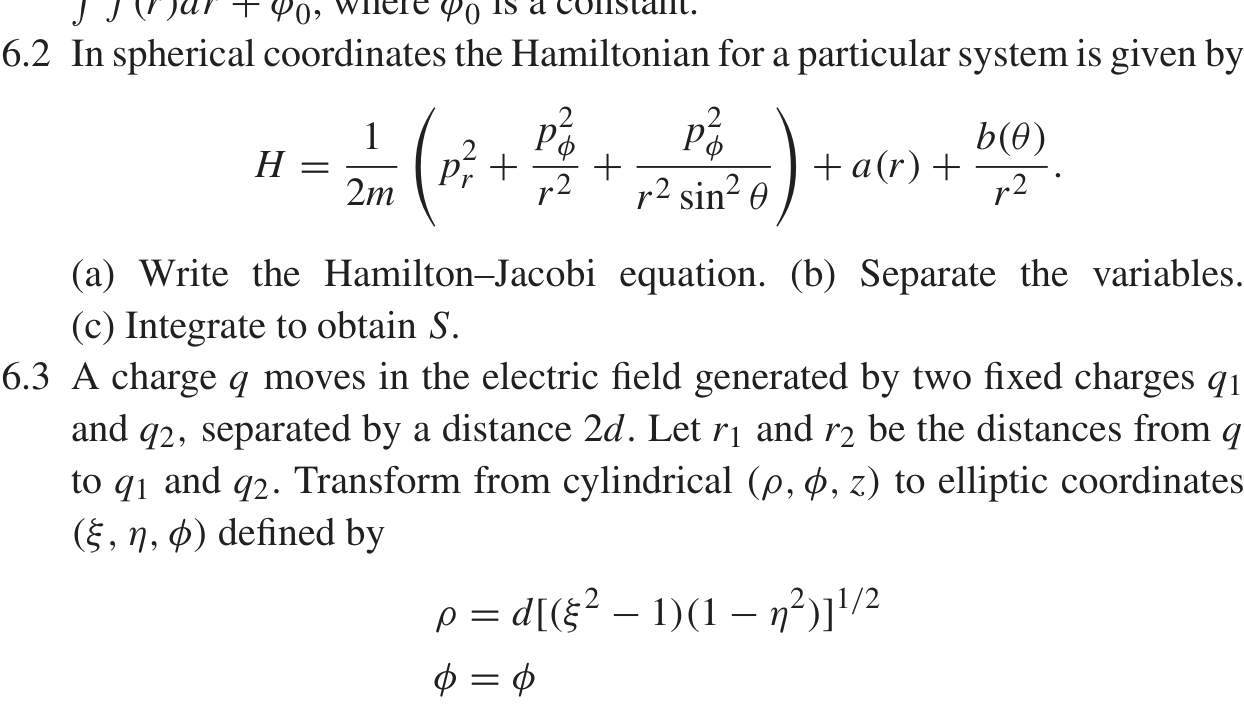
\includegraphics[width=0.55\linewidth]{../Figures/fig_6_1.png}
\caption{图 6.1}
\end{figure}

哈密顿量用 $p$ 和 $\phi$ 表示，其中 $p$ 是广义动量，$\phi$ 是珠子相对于圆环直径的角位置，如图所示。(a) 求出哈密顿主函数。(b) 求出 $\phi(t)$ 的积分表达式。

6.5 我们已把哈密顿主函数表示为 $S(q_i, \alpha_i, t)$。证明 $p_i$、$q_i$ 是正则变量，并回忆
\[
p_i = \frac{\partial S}{\partial q_i},
\]
\[
q_i = q_i(\alpha, \beta, t),
\]
其中
\[
\beta_i = Q_i = \frac{\partial S}{\partial \alpha_i},
\]
以及
\[
\alpha_i = P_i.
\]

\section*{6.6 一个质量为 $m$ 的质点在恒定引力场中被竖直向上抛出}

用哈密顿-雅可比方法求解该质点的运动问题。
